\documentclass[11pt]{article}

\usepackage{fullpage}
\usepackage{graphicx}
\title{INTEGRATION OF CLOUD COMPUTING WITH IOT}
\date{} %don't display the current date
\begin{document}
\maketitle
\section{INTRODUCTION}
It is important to explore the common features of the
technologies involved in the field of computing. Indeed, this is certainly the case with Cloud Computing and the Internet of
Things (IoT) – two paradigms that share many common
features. Cloud computing has altered the way in which technologies can be accessed, managed, and delivered. It is widely agreed that Cloud computing can be used for utility services in the future. Cloud computing has been involved in and encompassed various technologies such as grid, utility
computing virtualization, networking, and software services. Cloud computing provides services that make it possible
to share computing resources across the Internet. As such, it is not surprising that the origins of Cloud technologies lie in grid, utility computing virtualization, networking and software services, as well as distributed computing, and parallel computing.\\ On the other hand, the IoT can be considered both a dynamic and global networked infrastructure that manages self-configuring objects in a highly intelligent way. The IoT normally includes a number of objects with limited storage and computing capacity. It could well be said that Cloud computing and the IoT will be the future of the Internet and next-generation technologies. However, Cloud services are dependent on service providers which are extremely
interoperable, while IoT technologies are based on diversity
rather than interoperability.
 

\section{BASIC CONCEPTS}

\begin{itemize}
    \item[A.] CLOUD COMPUTING\\
    The National Institute of Standards and
Technology (NIST) has defined Cloud computing as "a model for enabling ubiquitous, convenient, on-demand network access to a shared pool of configurable computing resources (e.g., networks, servers, storage, applications, and services) that can be rapidly provisioned and released with minimal management effort or service provider interaction".
Cloud computing comprises four types of deployment models, three different service models, and five essential characteristics.\\
Cloud computing deployment models are most commonly
classified as belonging to the PUBLIC CLOUD, where resources
are made available to consumers over the Internet. Public
Clouds are generally owned by a profitable organisation (e.g.
Amazon). Conversely, the infrastructure of a PRIVATE CLOUD is commonly provided by a single organisation to serve
the particular purposes of its users(Microsoft
Private Cloud). HYBRID CLOUDS are a mixture of private and
public Clouds. This choice is provided for consumers as it
makes it possible to overcome some of the limitations of each
model. In contrast, a COMMUNITY CLOUD is a Cloud
infrastructure which is delivered to a group of users by a number of organizations that share the same need.\\
Services in Cloud computing are provided at three
different levels, namely: the Software as a Service (SaaS)
model, where software is delivered through the Internet to
users (e.g. GoogleApps); the Platform as a Service (PaaS)
model, which offers a higher level of an integrated environment
that can build, test, and deploy specific software (e.g.
Microsoft Azure); and finally, with the Infrastructure as a
Service (IaaS) model, infrastructure such as storage, hardware
and servers are delivered as a service (e.g. Amazon Web
Services). 
    \item[B.] INTERNET OF THINGS\\
All things in the IoT (smart devices, sensors, etc.) have their own identity. They are combined to form the communication network and will become actively participating objects. All IoT devices can be monitored, tracked and counted, which significantly decreases waste, loss, and cost.
According to the ITU (2012), the IoT is “a global
infrastructure for the Information Society, enabling advanced
services by interconnecting (physical and virtual) things based
on, existing and evolving, interoperable information and
communication technologies”. The IoT introduces a
variety of opportunities and applications. However, it faces
many challenges which could potentially hinder its successful implementation, such as data storage, heterogeneous resource-constrainted, scalability, Things, variable geospatial
deployment, and energy efficiency.
\item[C.] CLOUD-BASED INTERNET OF THINGS \\
The IoT and Cloud computing are both rapidly developing
services, and have their own unique characteristics. On the one
hand, the IoT approach is based on smart devices which
intercommunicate in a global network and dynamic
infrastructure. On the other hand, Cloud computing
comprises a massive network with unlimited storage
capabilities and computation power. Furthermore, it provides a
flexible, robust environment that allows for dynamic data
integration from various data sources. Cloud computing has
partially resolved most of the IoT issues. Indeed, the IoT and
Cloud are two comparatively challenging technologies and are
being combined in order to change the current and future
environment of internetworking services.
The Cloud-based Internet of Things is a platform which
allows for the smart usage of applications, information, and
infrastructure in a cost-effective way. While the IoT and Cloud
computing are different from each other, their features are
almost complementary.
  \begin{figure}[h]
  \centering
  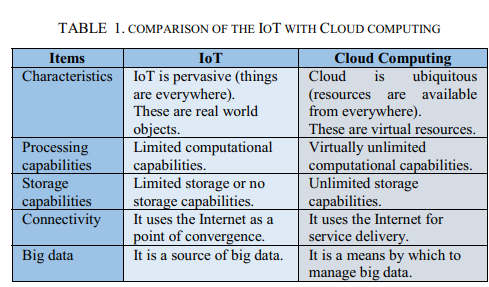
\includegraphics[width=0.7\textwidth]{fig/Screenshot (904).png}
  \end{figure}
\end{itemize}
\section{BENEFITS OF INTEGRATING IOT WITH CLOUD}\\

\begin{itemize}
  \item[1.] COMMUNICATION\\
Ubiquitous applications can be transmitted through the IoT, whilst automation can be utilised to facilitate low-cost data distribution and collection. The Cloud is an effective and economical solution which can be used to connect, manage, and track anything by using built-in apps and customised portals. It is worth declaring that, although the Cloud can greatly develop and facilitate the IoT interconnection, it still has weaknesses in certain areas. Thus, practical restrictions can appear when an enormous amount of data needs to be transferred . 
  \item[2.] STORAGE\\
As the IoT can be used on billions of devices, it comprises
a huge number of information sources, which generate an
enormous amount of semi-structured or non-structured data. This is known as Big Data, and has three characteristics: variety (e.g. data types), velocity (e.g. data generation
frequency), and volume (e.g. data size). The Cloud is
considered to be one of the most cost-effective and suitable
solutions when it comes to dealing with the enormous amount
of data created by the IoT. Moreover, it produces new chances
for data integration, aggregation, and sharing with third parties. 
  \item[3.]PROCESSING CAPABILITIES\\
IoT devices are characterised by limited processing
capabilities which prevent on-site and complex data
processing. Instead, gathered data is transferred to nodes that
have high capabilities. However, achieving scalability
remains a challenge without an appropriate underlying
infrastructure. Offering a solution, the Cloud provides
unlimited virtual processing capabilities and an on-demand
usage model. Predictive algorithms and data-driven
decisions making can be integrated into the IoT in order to
increase revenue and reduce risks at a lower cost.
  \item[4.] SCOPE\\
The Cloud-based IoT approach provides new applications and services based on the expansion of the Cloud through the IoT objects, which in turn allows the Cloud to work with a number of new real world scenarios, and leads to the emergence of new services.
\item[5.] NEW ABILITIES\\
The IoT is characterised by the heterogeneity of its devices,
protocols, and technologies. Hence, reliability, scalability,
interoperability, security, availability and efficiency can be
very hard to achieve. Integrating IoT into the Cloud resolves
most of these issues. It provides other features such as easeof-use and ease-of-access, with low deployment costs. 
\item[6.] NEW MODELS\\
• SaaS (Sensing as a Service), which allows access
to sensor data.
• EaaS (Ethernet as a Service), the main role of
which is to provide ubiquitous connectivity to control
remote devices.
• SAaaS (Sensing and Actuation as a Service),
which provides control logics automatically.
• IPMaaS (Identity and Policy Management as a Service), which provides access to policy and identitymanagement.
• DBaaS (Database as a Service), which provides
ubiquitous database management.
• SEaaS (Sensor Event as a Service), which
dispatches messaging services that are generated by
sensor events.
• SenaaS (Sensor as a Service), which provides
management for remote sensors.
• DaaS (Data as a Service), which provides
ubiquitous access to any type of data.
\end{itemize}
\section{CLOUD-BASED IOT ARCHITECTURE}\\
According to a number of previous studies, the well-known
IoT architecture is typically divided into three different layers: application, sensing and network layer. Most assume that the network layer is the Cloud layer, which realises the Cloudbased IoT architecture.
  \begin{figure}[h]
  \centering
  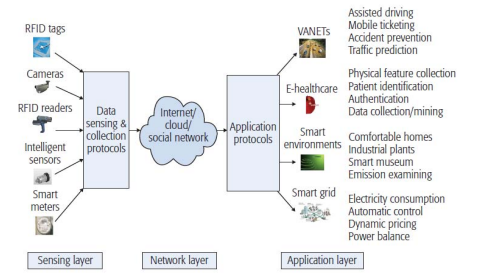
\includegraphics[width=0.6\textwidth]{fig/Screenshot (905).png}
  \end{figure}
The sensing layer is used to identify objects and gather
data, which is collected from the surrounding environment. In
contrast, the main objective of the network layer is to transfer the collected data to the Internet/Cloud. Finally, the application layer provides the interface to different services. 
\section{CLOUD-BASED IOT APPLICATIONS}
\begin{itemize}
\item[1.]HEALTHCARE: Cloud-based IoT develop and improve healthcare services and keep the field innovative (e.g. intelligent drug/medicine control, hospital management).
\item[2.]SMART CITIES: IoT technologies  will lead
to the generation of services that can communicate
with the surrounding environments (e.g. Smart
streetlights, Bigbelly, ShotSpotte).
\item[3.]VIDEO SURVEILLANCE: Intelligent video
surveillance will make it possible to manage, store, process video content and extract information from video sensors
easily and efficiently.(e.g. Wireless CCTV
Cameras). 
\item[4.]AUTOMOTIVE AND SMART MOBILITY: The integration of Cloud computing into The Global Positioning System (GPS) represents a opportunity to solve many of the existing challenges (e.g. traffic state prediction & notification, remote vehicles).
\item[5.]SMART ENERGY AND SMART GRID: Cloud computing and the IoT can work together effectively to provide consumers with smart management of energy consumption (e.g. smart
meters, smart appliances, renewable energy resources). 
\item[6.]SMART LOGISTICS: It allows for, and eases, the automated management of goods flow between producers and consumers, while simultaneously enabling the tracking of
goods in transit (e.g. logistics industry, tracking
shipments).   
\end{itemize}
\section{CHALLENGES FACING CLOUD-BASED IOT INTEGRATION}
\begin{itemize}
\item[1.]SECURITY AND PRIVACY\\
Important issues which has not yet been resolved is how to provide appropriate authorisation rules and policies while ensuring that only authorised users have access to the sensitive data.Sensitive information leakage can occur due to the multi-tenancy. Moreover, public key cryptography cannot be applied to all layers because of the processing power constraints imposed by IoT objects.
\item[2.]HETEROGENEITY\\
 Cloud platforms suffer from heterogeneity issues; for instance, Cloud services generally come with proprietary interfaces, thus allowing for resource integration based on specific providers. In addition, the heterogeneity challenge can be exacerbated when end-users adopt multi-Cloud approaches, and thus services will depend on multiple providers to improve application performance and resilience.
\item[3.]BIG DATA\\
Finding a perfect data management solution which will allow the Cloud to manage massive amounts of data is still a big issue. Furthermore, data integrity is a vital element, not only because of its effect on the service’s quality, but also because of security and privacy issues, the majority of which relate to outsourced data. 
\item[4.]PERFORMANCE\\
 The key issue is obtaining adequate network performance in order to transfer data to Cloud environments. In a number of scenarios, services and data provision should be achieved with high reactivity. This is because timeliness might be affected by unpredictable matters and real-time applications are very sensitive to performance efficiency.
 \item[5.]LEGAL ASPECTS \\
 Legal aspects have been very significant in recent research
concerning certain applications. For instance, service providers must adapt to various international regulations. On the other hand, users should give donations in order to contribute to data collection. 

 \item[6.]MONITORING \\
 Monitoring is a primary action in Cloud Computing when it
comes to performance, managing resources, capacity planning,
security, SLAs, and for troubleshooting. As a result, the Cloudbased IoT approach inherits the same monitoring demands
from the Cloud, although there are still some related challenges that are impacted by velocity, volume, and variety
characteristics of the IoT. 
 \item[7.]LARGE SCALE\\
The large scale of the systems raises many
new issues that are difficult to overcome. For instance,
achieving computational capability and storage capacity
requirements is becoming difficult. Moreover, the monitoring
process has made the distribution of the IoT devices more
difficult, as IoT devices have to face connectivity issues and
latency dynamics. 


\end{itemize}

\section{OPEN ISSUES AND RESEARCH DIRECTIONS}
\begin{itemize}
\item[1.]STANDARDISATION\\
Many studies have highlighted the issues of lack of
standards, which is considered critical in relation to the Cloudbased IoT paradigm. Architectures, standard protocols, and APIs are required to allow for interconnection between heterogeneous smart things and the generation of new services, which make up the Cloudbased IoT paradigm.
\item[2.]FOG COMPUTING\\
Fog can essentially be considered an extension of Cloud Computing which acts as an intermediate between the edge of the network and the Cloud; indeed, it works with latency-sensitive applications that require other nodes to satisfy their delay requirements. Although storage, computing, and
networking are the main resources of both Fog and the Cloud,
the Fog has certain features, such as location awareness and
edge location, that provide geographical distribution, and low
latency; moreover, there are a large nodes; this is in contrast
with the Cloud, which is supported for real-time interaction
and mobility. 
\item[3.]CLOUD CAPABILITIES\\
As in any networked environment, security is considered to
be one of the main issues of the Cloud-based IoT paradigm.
There are more chances of attacks on both the IoT and the
Cloud side. In the IoT context, data integrity, confidentiality
and authenticity can be guaranteed by encryption. However,
insider attacks cannot be resolved and it is also hard to use the IoT on devices with limited capabilities.
\item[4.]SLA ENFORCEMENT\\
Ensuring a specific Quality of Service (QoS) level regarding Cloud resources by depending on a single provider raises many issues. Thus, multiple Cloud providers may be required to avoid SLA violations. However, dynamically choosing the most appropriate mixture of Cloud providers still represents an open issue due to time, costs, and heterogeneity of QoS management support .
\item[5.]BIG DATA\\
Big Data is considered a critical open issue, and
one in need of more research. The Cloud-based IoT approach
involves the management and processing of huge amounts of
data stemming from various locations and from heterogeneous
sources; indeed, in the Cloud-based IoT, many applications
need complicated tasks to be performed in real-time. 
\item[6.]ENERGY EFFICIENCY\\
Recent Cloud-based IoT applications quickly consumes the node energy. Several directions have been suggested to overcome this issue, such as compression technologies, efficient data transmission; and data caching techniques for reusing collected data with time-insensitive application. 
\item[7.]SECURITY AND PRIVACY \\
Adapting to different threats from hackers is an issue.
Moreover, another problem is providing the appropriate
authorisation rules and policies while ensuring that only
authorised users have access to sensitive data; this is crucial for preserving users’ privacy, specifically when data integrity must be guaranteed. 
\end{itemize}

\section{CONCLUSION}\\
The IoT is becoming an increasingly ubiquitous computing
service which requires huge volumes of data storage and
processing capabilities. The IoT has limited capabilities in
terms of processing power and storage, while there also exist
consequential issues such as security, privacy, performance,
and reliability; As such, the integration of the Cloud into the
IoT is very beneficial in terms of overcoming these challenges.
In this paper, we presented the need for the creation of the
Cloud-based IoT approach. Discussion also focused on the
Cloud-based IoT architecture, different applications scenarios,
challenges facing the successful integration, and open research
directions. In future work, a number of case studies will be
carried out to test the effectiveness of the Cloud-based IoT
approach in healthcare applications. 
\\
\\
\\
\\
\\
\\
\section*{SUBMISSION MADE BY:}\\
D M SHALINI JAYASRI\\
21011101038\\
AI-DS-A






\end{document}